\documentclass[10.5pt]{article}
\usepackage{amsmath,amssymb,amsthm}
\usepackage{listings}
\usepackage{graphicx}
\usepackage[shortlabels]{enumitem}
\usepackage{tikz}
\usepackage[margin=1in]{geometry}
\usepackage{fancyhdr}
\usepackage{epsfig} %% for loading postscript figures
\usepackage{amsmath}
\usepackage{float}
\usepackage{amssymb}
\usepackage{caption}
\usepackage{subfigure}
\usepackage{graphics}
\usepackage{titlesec}
\usepackage{mathrsfs}
\usepackage{amsfonts}
\usepackage{indentfirst}
\usepackage{fontspec}
\usepackage{xcolor}
\renewcommand{\baselinestretch}{1.2}%Adjust Line Spacing
%\geometry{left=2.0cm,right=2.0cm,top=2.0cm,bottom=2.0cm}% Adjust Margins of the File
\usepackage{tikz-qtree}
\usetikzlibrary{graphs}
\tikzset{every tree node/.style={minimum width=2em,draw,circle},
    blank/.style={draw=none},
    edge from parent/.style=
    {draw,edge from parent path={(\tikzparentnode) -- (\tikzchildnode)}},
    level distance=1.2cm}
\setlength{\parindent}{0pt}
%\setlength{\parskip}{5pt plus 1pt}
\setlength{\headheight}{13.6pt}
\newcommand\question[2]{\vspace{.25in}\hrule\textbf{#1: #2}\vspace{.5em}\hrule\vspace{.10in}}
\renewcommand\part[1]{\vspace{.10in}\textbf{(#1)}}
\newcommand\algorithm{\vspace{.10in}\textbf{Algorithm: }}
\newcommand\correctness{\vspace{.10in}\textbf{Correctness: }}
\newcommand\runtime{\vspace{.10in}\textbf{Running time: }}
\pagestyle{fancyplain}
% Create horizontal rule command with an argument of height
\newcommand{\horrule}[1]{\rule{\linewidth}{#1}}
% Set the title here
\title{
    \normalfont \normalsize
    \textsc{ShanghaiTech University} \\ [25pt]
    \horrule{0.5pt} \\[0.4cm] % Thin top horizontal rule
    \huge CS101 Algorithms and Data Structures\\ % The assignment title
    \LARGE Fall 2021\\
    \LARGE Homework 5\\
    \horrule{2pt} \\[0.5cm] % Thick bottom horizontal rule
}
% wrong usage of \author, never mind
\author{}
\date{Due date: 23:59, October 31, 2021}

% set the header and footer
\pagestyle{fancy}
\lhead{CS101 Algorithms and Data Structures}
\chead{Homework 5}
\rhead{Due date: 23:59, October 31, 2021}
\cfoot{\thepage}
\renewcommand{\headrulewidth}{0.4pt}

% special settings for the first page
\fancypagestyle{firstpage}
{
    \renewcommand{\headrulewidth}{0pt}
    \fancyhf{}
    \fancyfoot[C]{\thepage}
}

% Add the support for auto numbering
% use \problem{title} or \problem[number]{title} to add a new problem
% also \subproblem is supported, just use it like \subsection
\newcounter{ProblemCounter}
\newcounter{oldvalue}
\newcommand{\problem}[2][-1]{
    \setcounter{oldvalue}{\value{secnumdepth}}
    \setcounter{secnumdepth}{0}
    \ifnum#1>-1
        \setcounter{ProblemCounter}{0}
    \else
        \stepcounter{ProblemCounter}
    \fi
    \section{Problem \arabic{ProblemCounter}: #2}
    \setcounter{secnumdepth}{\value{oldvalue}}
}
\newcommand{\subproblem}[1]{
    \setcounter{oldvalue}{\value{section}}
    \setcounter{section}{\value{ProblemCounter}}
    \subsection{#1}
    \setcounter{section}{\value{oldvalue}}
}
\definecolor{blve}{rgb}{0.3372549 , 0.61176471, 0.83921569}
\definecolor{gr33n}{rgb}{0.29019608, 0.7372549 , 0.64705882}
\makeatletter
\lst@InstallKeywords k{class}{classstyle}\slshape{classstyle}{}ld
\makeatother
\lstset{language=C++,
	basicstyle=\ttfamily,
	keywordstyle=\color{blve}\ttfamily,
	stringstyle=\color{red}\ttfamily,
	commentstyle=\color{green}\ttfamily,
	morecomment=[l][\color{magenta}]{\#},
	classstyle = \bfseries\color{gr33n}, 
	tabsize=4
}


\begin{document}

\maketitle
\thispagestyle{firstpage}
%\newpage
\vspace{3ex}

\begin{enumerate}
\item Please write your solutions in English. 

\item Submit your solutions to gradescope.com.  

\item Set your FULL Name to your Chinese name and your STUDENT ID correctly in Account Settings. 

\item If you want to submit a handwritten version, scan it clearly. Camscanner is recommended. 

\item When submitting, match your solutions to the according problem numbers correctly. 

\item No late submission will be accepted.

\item Violations to any of the above may result in zero grade. 
\end{enumerate}
\newpage


%---------------------------------------------------------------
\problem{Multiple Choices}
Multiple Choices: Each question has one or more correct answer(s). Select all the correct answer(s). For each question, you get $0$ point if you select one or more wrong answers, but you get half points if you select a non-empty subset of the correct answers.\\
\textit{Note that you should write you answers of Problem 1 in the table below.}
\begin{table}[htbp]
\begin{tabular}{|p{1.5cm}|p{1.5cm}|p{1.5cm}|}
\hline 
Q(1) & Q(2) & Q(3) \\
\hline 
&&\\ 
\hline 
\end{tabular} 
\end{table} \\
%%%%% (1)
(1) Which of the following are true about Binary Trees? (2pts) \\
A. Every full binary tree is also a complete binary tree. \\
B. A full binary tree with n nodes has height of $O(\ln{n})$. \\
C. A complete binary tree with n leaves has exactly $2n-1$ nodes.\\
D. A full binary tree with n leaves has exactly $2n-1$ nodes.\\
E. None of the above.

~\\
%%%%% (2)
(2) Which traversals of the left tree and right tree, will produce the same sequence node name? (2pts) \\
\begin{minipage}{1\textwidth}
\centering
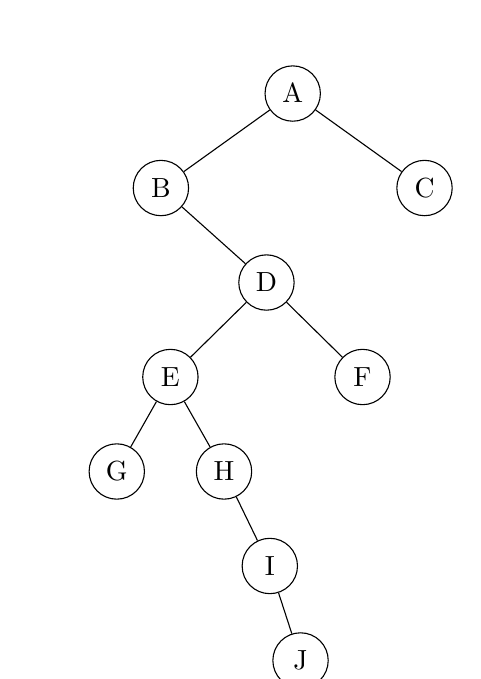
\begin{tikzpicture}
\Tree
[.A
    [.B
        \edge[blank]; \node[blank]{};
        \edge[];[.D
            \edge[];[.E
                \edge[];[.G ]
                \edge[];[.H
                    \edge[blank]; \node[blank]{};
                    \edge[];[.I 
                        \edge[blank]; \node[blank]{};
                        \edge[];[.J
                        ] 
                    ]
                ]
            ]
            \edge[]; [.F
            ]
        ]
    ]
    [.C
    ]
]
\end{tikzpicture}
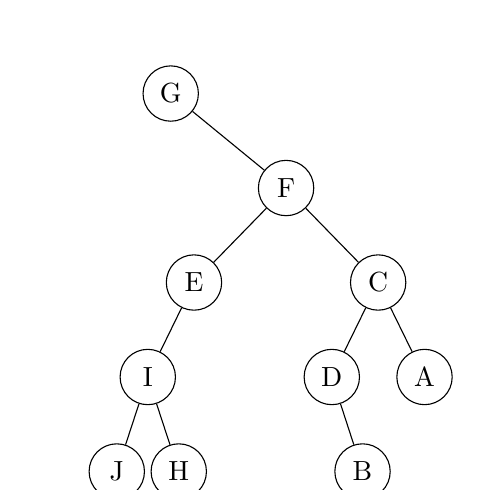
\begin{tikzpicture}
\Tree
[.G
    \edge[blank]; \node[blank]{};
    \edge[]; [.F
        \edge[]; [.E 
            \edge[];[.I 
                \edge[];[.J ]
                \edge[];[.H ]
            ]
            \edge[blank]; \node[blank]{};
        ]
        \edge[]; [.C 
            \edge[]; [.D
                \edge[blank]; \node[blank]{};
                \edge[];[.B ]  
            ]
            \edge[]; [.A ]
        ] 
    ]
]
\end{tikzpicture}
\end{minipage} \\
A. left: In-order, right: In-order \\
B. left: Pre-order, right: Pre-order \\
C. left: Post-order, right: Post-order \\
D. left: Post-order, right: In-order
~\\

%%%%% (2)
(3) Which of the following statements about the binary heap is \textbf{not} true? Note that binary heaps mentioned in this problem are implemented by complete binary trees. (2pts) \\
A. There exists a heap with seven distinct elements so that the in-order traversal gives the element in sorted order. \\
B. If item A is an ancestor of item B in a heap (used as a Priority Queue) then it must be the case that the Insert operation for item A occurred before the \textbf{Insert} operation for item B.\\
C. If array A is sorted from smallest to largest then A (excluding A[0]) corresponds to a min-heap. \\
D. None of the above. 

\pagebreak
% -------------------------------------------------------------------------
\problem{Construct a Heap}
(1) Suppose we construct a min-heap from the following initial heap using Floyd's method. After the construction is completed, what should this heap look like? Please draw it as a binary tree. (5pts) \\

\begin{minipage}{1\textwidth}
\centering
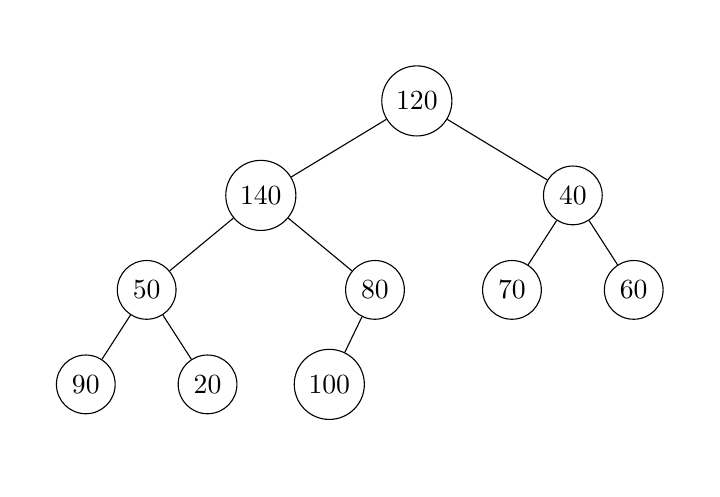
\begin{tikzpicture}
\Tree
[.120
[.140
\edge[]; [.50
\edge[]; [.90
\edge[blank]; \node[blank]{};
\edge[blank]; \node[blank]{};
]
\edge[]; [.20
\edge[blank]; \node[blank]{};
\edge[blank]; \node[blank]{};
]
]
\edge[]; [.80
\edge[]; [.100
\edge[blank]; \node[blank]{};
\edge[blank]; \node[blank]{};
]
\edge[blank]; \node[blank]{};
]
]
[.40
% \edge[blank]; \node[blank]{};
\edge[]; [.70
\edge[blank]; \node[blank]{};
\edge[blank]; \node[blank]{};
]
\edge[]; [.60
\edge[blank]; \node[blank]{};
\edge[blank]; \node[blank]{};
]
]
]
\end{tikzpicture}
\end{minipage}%
\vspace{150pt}

(2) Suppose we delete the root from the heap constructed in (1). What will be the post-order traversal of the new heap? (2pts) \\
\textbf{Your answer:} \underline{\hspace{60pt}}.\\

(3) Suppose there is a binary tree with the same post-order traversal of the heap in (2), and the binary tree has an \textbf{in-order} traversal of $120,140,80,90,40,60,50,100,70$. Please draw this binary tree below. (5pts) 

\pagebreak

%------------------------------------------------------------------
\problem{Heap Sort}
\paragraph{}
You are given such a max heap like this:

\begin{minipage}{1\textwidth}
\centering
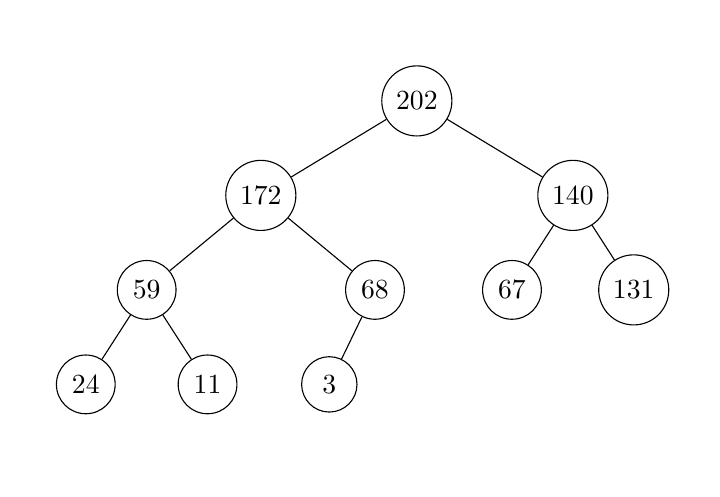
\begin{tikzpicture}
\Tree
[.202
    [.172
        \edge[]; [.59
            \edge[]; [.24
                \edge[blank]; \node[blank]{};
                \edge[blank]; \node[blank]{};
            ]
            \edge[]; [. 11
                \edge[blank]; \node[blank]{};
                \edge[blank]; \node[blank]{};
            ]
        ]
        \edge[]; [.68
            \edge[]; [.3
                \edge[blank]; \node[blank]{};
                \edge[blank]; \node[blank]{};
            ]
            \edge[blank]; \node[blank]{};
        ]
    ]
    [.140
    % \edge[blank]; \node[blank]{};
        \edge[]; [.67
            \edge[blank]; \node[blank]{};
            \edge[blank]; \node[blank]{};
        ]
        \edge[]; [.131
            \edge[blank]; \node[blank]{};
            \edge[blank]; \node[blank]{};
        ]
    ]
]
\end{tikzpicture}
\end{minipage}%

Then you need to use array method to show each step of heap sort in increasing order. Fill in the value in the table below. Notice that the value we have put is the step of each value sorted successfully. For each step, you should always make you heap satisfies the requirement of max heap property. (10pts) 

\begin{table}[!hbtp]
\centering
\resizebox{\textwidth}{!}{%
    \begin{tabular}{|c|c|c|c|c|c|c|c|c|c|c|c|}
        \hline
        index & 0 & 1 & 2 & 3 & 4 & 5 & 6 & 7 & 8 & 9 & 10 \\ \hline
        value & $\quad $ & $\quad $ & $\quad $ &$\quad $  &$\quad $  & $\quad $ &$\quad $  &$\quad $  & $\quad $ &$\quad $  &$\quad $  \\ \hline
    \end{tabular}%
}
\caption{The original array to represent max heap.}
\label{}
\end{table}
\begin{table}[!hbtp]
\centering
\resizebox{\textwidth}{!}{%
    \begin{tabular}{|c|c|c|c|c|c|c|c|c|c|c|c|}
        \hline
        index & 0 & 1 & 2 & 3 & 4 & 5 & 6 & 7 & 8 & 9 & 10 \\ \hline
        value & $\quad $ &$\quad $  &$\quad $  &$\quad $  &$\quad $  & $\quad $ &$\quad $  &$\quad $  &$\quad $  &$\quad $  & \color{blue}202 \\ \hline
    \end{tabular}%
}
\caption{First value is successfully sorted.}
\label{}
\end{table}
\begin{table}[h]
\centering
\resizebox{\textwidth}{!}{%
    \begin{tabular}{|c|c|c|c|c|c|c|c|c|c|c|c|}
        \hline
        index & 0 & 1 & 2 & 3 & 4 & 5 & 6 & 7 & 8 & 9 & 10 \\ \hline
        value &$\quad $  &$\quad $ & $\quad $ & $\quad $ & $\quad $ & $\quad $ & $\quad $ & $\quad $& $\quad $ & \color{blue}172 & \color{blue}202 \\ \hline
    \end{tabular}%
}
\caption{Second value is successfully sorted.}
\label{}
\end{table}
\begin{table}[!hbtp]
\centering
\resizebox{\textwidth}{!}{%
    \begin{tabular}{|c|c|c|c|c|c|c|c|c|c|c|c|}
        \hline
        index & 0 & 1 & 2 & 3 & 4 & 5 & 6 & 7 & 8 & 9 & 10 \\ \hline
        value &$\quad $  & $\quad $ & $\quad $ & $\quad $ & $\quad $ & $\quad $ & $\quad $ & $\quad $ & \color{blue}140 & \color{blue}172 & \color{blue}202  \\ \hline
    \end{tabular}%
}
\caption{Third value is successfully sorted.}
\label{}
\end{table}
\begin{table}[!hbtp]
\centering
\resizebox{\textwidth}{!}{%
    \begin{tabular}{|c|c|c|c|c|c|c|c|c|c|c|c|}
        \hline
        index & 0 & 1 & 2 & 3 & 4 & 5 & 6 & 7 & 8 & 9 & 10 \\ \hline
        value &$\quad $  & $\quad $ & $\quad $ & $\quad $ & $\quad $ & $\quad $ & $\quad $ & \color{blue}131 & \color{blue}140 & \color{blue}172 & \color{blue}202 \\ \hline
    \end{tabular}%
}
\caption{Fourth value is successfully sorted.}
\label{}
\end{table}
\begin{table}[!hbtp]
\centering
\resizebox{\textwidth}{!}{%
    \begin{tabular}{|c|c|c|c|c|c|c|c|c|c|c|c|}
        \hline
        index & 0 & 1 & 2 & 3 & 4 & 5 & 6 & 7 & 8 & 9 & 10 \\ \hline
        value & $\quad $ & $\quad $ & $\quad $ & $\quad $ & $\quad $ & $\quad $ & \color{blue}68 & \color{blue}131 & \color{blue}140 & \color{blue}172 & \color{blue}202 \\ \hline
    \end{tabular}%
}
\caption{Fifth value is successfully sorted.}
\label{}
\end{table}
\begin{table}[!hbtp]
\centering
\resizebox{\textwidth}{!}{%
    \begin{tabular}{|c|c|c|c|c|c|c|c|c|c|c|c|}
        \hline
        index & 0 & 1 & 2 & 3 & 4 & 5 & 6 & 7 & 8 & 9 & 10 \\ \hline
        value & $\quad $ & $\quad $ & $\quad $& $\quad $ & $\quad $ & \color{blue}67 & \color{blue}68 & \color{blue}131 & \color{blue}140 & \color{blue}172 & \color{blue}202 \\ \hline
    \end{tabular}%
}
\caption{Sixth value is successfully sorted.}
\label{}
\end{table}
\begin{table}[!hbtp]
\centering
\resizebox{\textwidth}{!}{%
    \begin{tabular}{|c|c|c|c|c|c|c|c|c|c|c|c|}
        \hline
        index & 0 & 1 & 2 & 3 & 4 & 5 & 6 & 7 & 8 & 9 & 10 \\ \hline
        value & $\quad $ & $\quad $ & $\quad $ & $\quad $ & \color{blue}59 & \color{blue}67 & \color{blue}68 & \color{blue}131 & \color{blue}140 & \color{blue}172 & \color{blue}202 \\ \hline
    \end{tabular}%
}
\caption{Seventh value is successfully sorted.}
\label{}
\end{table}
\begin{table}[!hbtp]
\centering
\resizebox{\textwidth}{!}{%
    \begin{tabular}{|c|c|c|c|c|c|c|c|c|c|c|c|}
        \hline
        index & 0 & 1 & 2 & 3 & 4 & 5 & 6 & 7 & 8 & 9 & 10 \\ \hline
        value & $\quad $ & $\quad $ & $\quad $ & \color{blue}24 & \color{blue}59 & \color{blue}67 & \color{blue}68 & \color{blue}131 & \color{blue}140 & \color{blue}172 & \color{blue}202 \\ \hline
    \end{tabular}%
}
\caption{Eighth value is successfully sorted.}
\label{}
\end{table}
\begin{table}[!hbtp]
\centering
\resizebox{\textwidth}{!}{%
    \begin{tabular}{|c|c|c|c|c|c|c|c|c|c|c|c|}
        \hline
        index & 0 & 1 & 2 & 3 & 4 & 5 & 6 & 7 & 8 & 9 & 10 \\ \hline
        value & $\quad $ & $\quad $ & \color{blue}11 & \color{blue}24 & \color{blue}59 & \color{blue}67 & \color{blue}68 & \color{blue}131 & \color{blue}140 & \color{blue}172 & \color{blue}202 \\ \hline
    \end{tabular}%
}
\caption{Last 2 values are successfully sorted.}
\label{}
\end{table}

 
\newpage
%%%%%%%%%%%%%%%%%%%%%%%%%%%%%%%%%%%%%%%%%%%% Start of Problem 4 %%%%%%%%%%%%%%%%%%%%%%%%%%%%%%%%%%%%%%%%%%%%%%%
\problem{$i$-Heap}
\paragraph{}
In class, Prof. Zhang has mentioned the method of the array storage of a binary heap. In order to have a better view of heap, we decide to extend the idea of a binary heap to $i$-heap. In other words, each node in the heap now has at most $i$ children instead of just two, which is stored in a complete binary tree.

For example, the following heap is a 3-heap.
~\\

\begin{minipage}{1\textwidth}
	\centering
	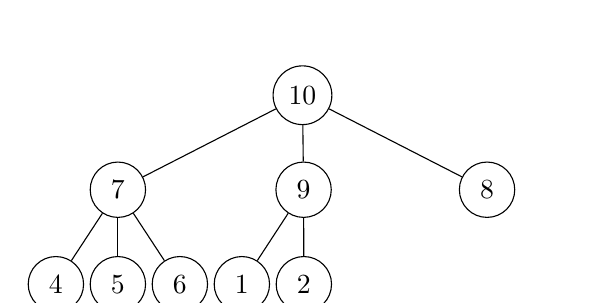
\begin{tikzpicture}
	\Tree
	[.10
		[.7
			\edge[]; [.4
			]
			\edge[]; [.5
			]
			\edge[]; [.6
			]
		]
		[.9
			\edge[]; [.1 
			]
			\edge[]; [.2 
			]
			\edge[blank]; \node[blank]{};
		]
		[.8
			\edge[blank]; \node[blank]{};
			\edge[blank]; \node[blank]{};
			\edge[blank]; \node[blank]{};
		]
	]
	\end{tikzpicture}
\end{minipage}%

~\\

%%%%% (1)
(1) (4pts) If you are given the node with index $x$, what is the index of its parent and its $y$th child ($1 \leq y \leq i$)?

\textbf{Notice: }We assume the root is kept in $A[1]$. For your final answer, please represent it in terms of $i$, $x$ and $y$. Please use flooring or ceiling to ensure that your final answer is as tight as possible if you need, i.e. $\lfloor m \rfloor$, $\lceil m \rceil$.
~\\

%%%%%%%%%%%%%%%%%%%%%%%%%%%%%%%%%%%%%%%%% START YOUR SOLUTION %%%%%%%%%%%%%%%%%%%%%%%%%%%%%%%%%%%%%%%%%
%~\\
%\textbf{Solution:}

%%%%%%%%%%%%%%%%%%%%%%%%%%%%%%%%%%%%%%%%% END YOUR SOLUTION %%%%%%%%%%%%%%%%%%%%%%%%%%%%%%%%%%%%%%%%%
\newpage
%%%%% (2)
(2) (4pts) What is the height of a $i$-heap of $n$ elements? Please show your steps.

\textbf{Notice: }For your final answer, please represent it in terms of $i$ and $n$. Please use flooring or ceiling to ensure that your final answer is as tight as possible if you need, i.e. $\lfloor m \rfloor$, $\lceil m \rceil$.
~\\

%%%%%%%%%%%%%%%%%%%%%%%%%%%%%%%%%%%%%%%%% START YOUR SOLUTION %%%%%%%%%%%%%%%%%%%%%%%%%%%%%%%%%%%%%%%%%
%~\\
%\textbf{Solution:}

%%%%%%%%%%%%%%%%%%%%%%%%%%%%%%%%%%%%%%%%% END YOUR SOLUTION %%%%%%%%%%%%%%%%%%%%%%%%%%%%%%%%%%%%%%%%%
\newpage
(3) (4pts) Now we want to study which value of $i$ can minimize the comparison complexity of heap-sort. For heap-sort, given a built heap, the worst-case number of comparisons is $\Theta(nhi)$, where $h=\Theta(\log_in)$ is the height of the heap. Suppose the worst-case number of comparisons is $T(n,i)$. You need to do: 

\begin{itemize}
	\item{Explain why $T(n,i) = \Theta(nhi)$.}
	\item{Suppose $n$ is fixed, solve for $i$ so that $T(n,i)$ is minimized.}
\end{itemize}

\textbf{Notice: } $i$ is an integer actually. In this problem, we only consider the complexity of comparison, not the accurate number of comparison.

%%%%%%%%%%%%%%%%%%%%%%%%%%%%%%%%%%%%%%%%% START YOUR SOLUTION %%%%%%%%%%%%%%%%%%%%%%%%%%%%%%%%%%%%%%%%%
%~\\
%\textbf{Solution:}

%%%%%%%%%%%%%%%%%%%%%%%%%%%%%%%%%%%%%%%%% END YOUR SOLUTION %%%%%%%%%%%%%%%%%%%%%%%%%%%%%%%%%%%%%%%%%
\newpage
%%%%% (4)
(4) (5pts) TA Xiaozhang Master has a new idea that if $i = 1$, we only need to do the \texttt{BUILD-HEAP} operation to get a sorted array. Since we know from the lecture that \texttt{BUILD-HEAP} takes $O(n)$ time, he thinks it can actually sort in $O(n)$ time! \\

Now you are the student of TA Xiaozhang Master, and you need to judge his statement is true or false. 
\begin{itemize}
	\item{If his statement is true, please explain the reason and prove its correctness.}
	\item{If his statement is false, please help him find the fallacy in his argument with your own reason. In the heap-sort he proposes, what sorting algorithm is actually performed? What is the worst running time of such a sorting algorithm?}
\end{itemize}
%%%%%%%%%%%%%%%%%%%%%%%%%%%%%%%%%%%%%%%%% START YOUR SOLUTION %%%%%%%%%%%%%%%%%%%%%%%%%%%%%%%%%%%%%%%%%
%~\\
%\textbf{Solution:}



























%%%%%%%%%%%%%%%%%%%%%%%%%%%%%%%%%%%%%%%%% END YOUR SOLUTION %%%%%%%%%%%%%%%%%%%%%%%%%%%%%%%%%%%%%%%%%
%%%%%%%%%%%%%%%%%%%%%%%%%%%%%%%%%%%%%%%%%%%% End of Problem 4 %%%%%%%%%%%%%%%%%%%%%%%%%%%%%%%%%%%%%%%%%%%%%%%
\end{document}

\end{document}